%\section{Морфологическая и семантическая разметка корпуса ВепКар} \label{sect_exp_tag_vepkar}

\subsection{Организация данных и разметка текста в корпусе ВепКар} \label{sect_exp_tag_vepkar_data_org}

Одно из направлений работ в рамках развития Открытого корпуса вепсского и карельского языков связано с автоматизацией грамматической разметки вепсских и карельских текстов. 

\begin{figure}
    \centering
    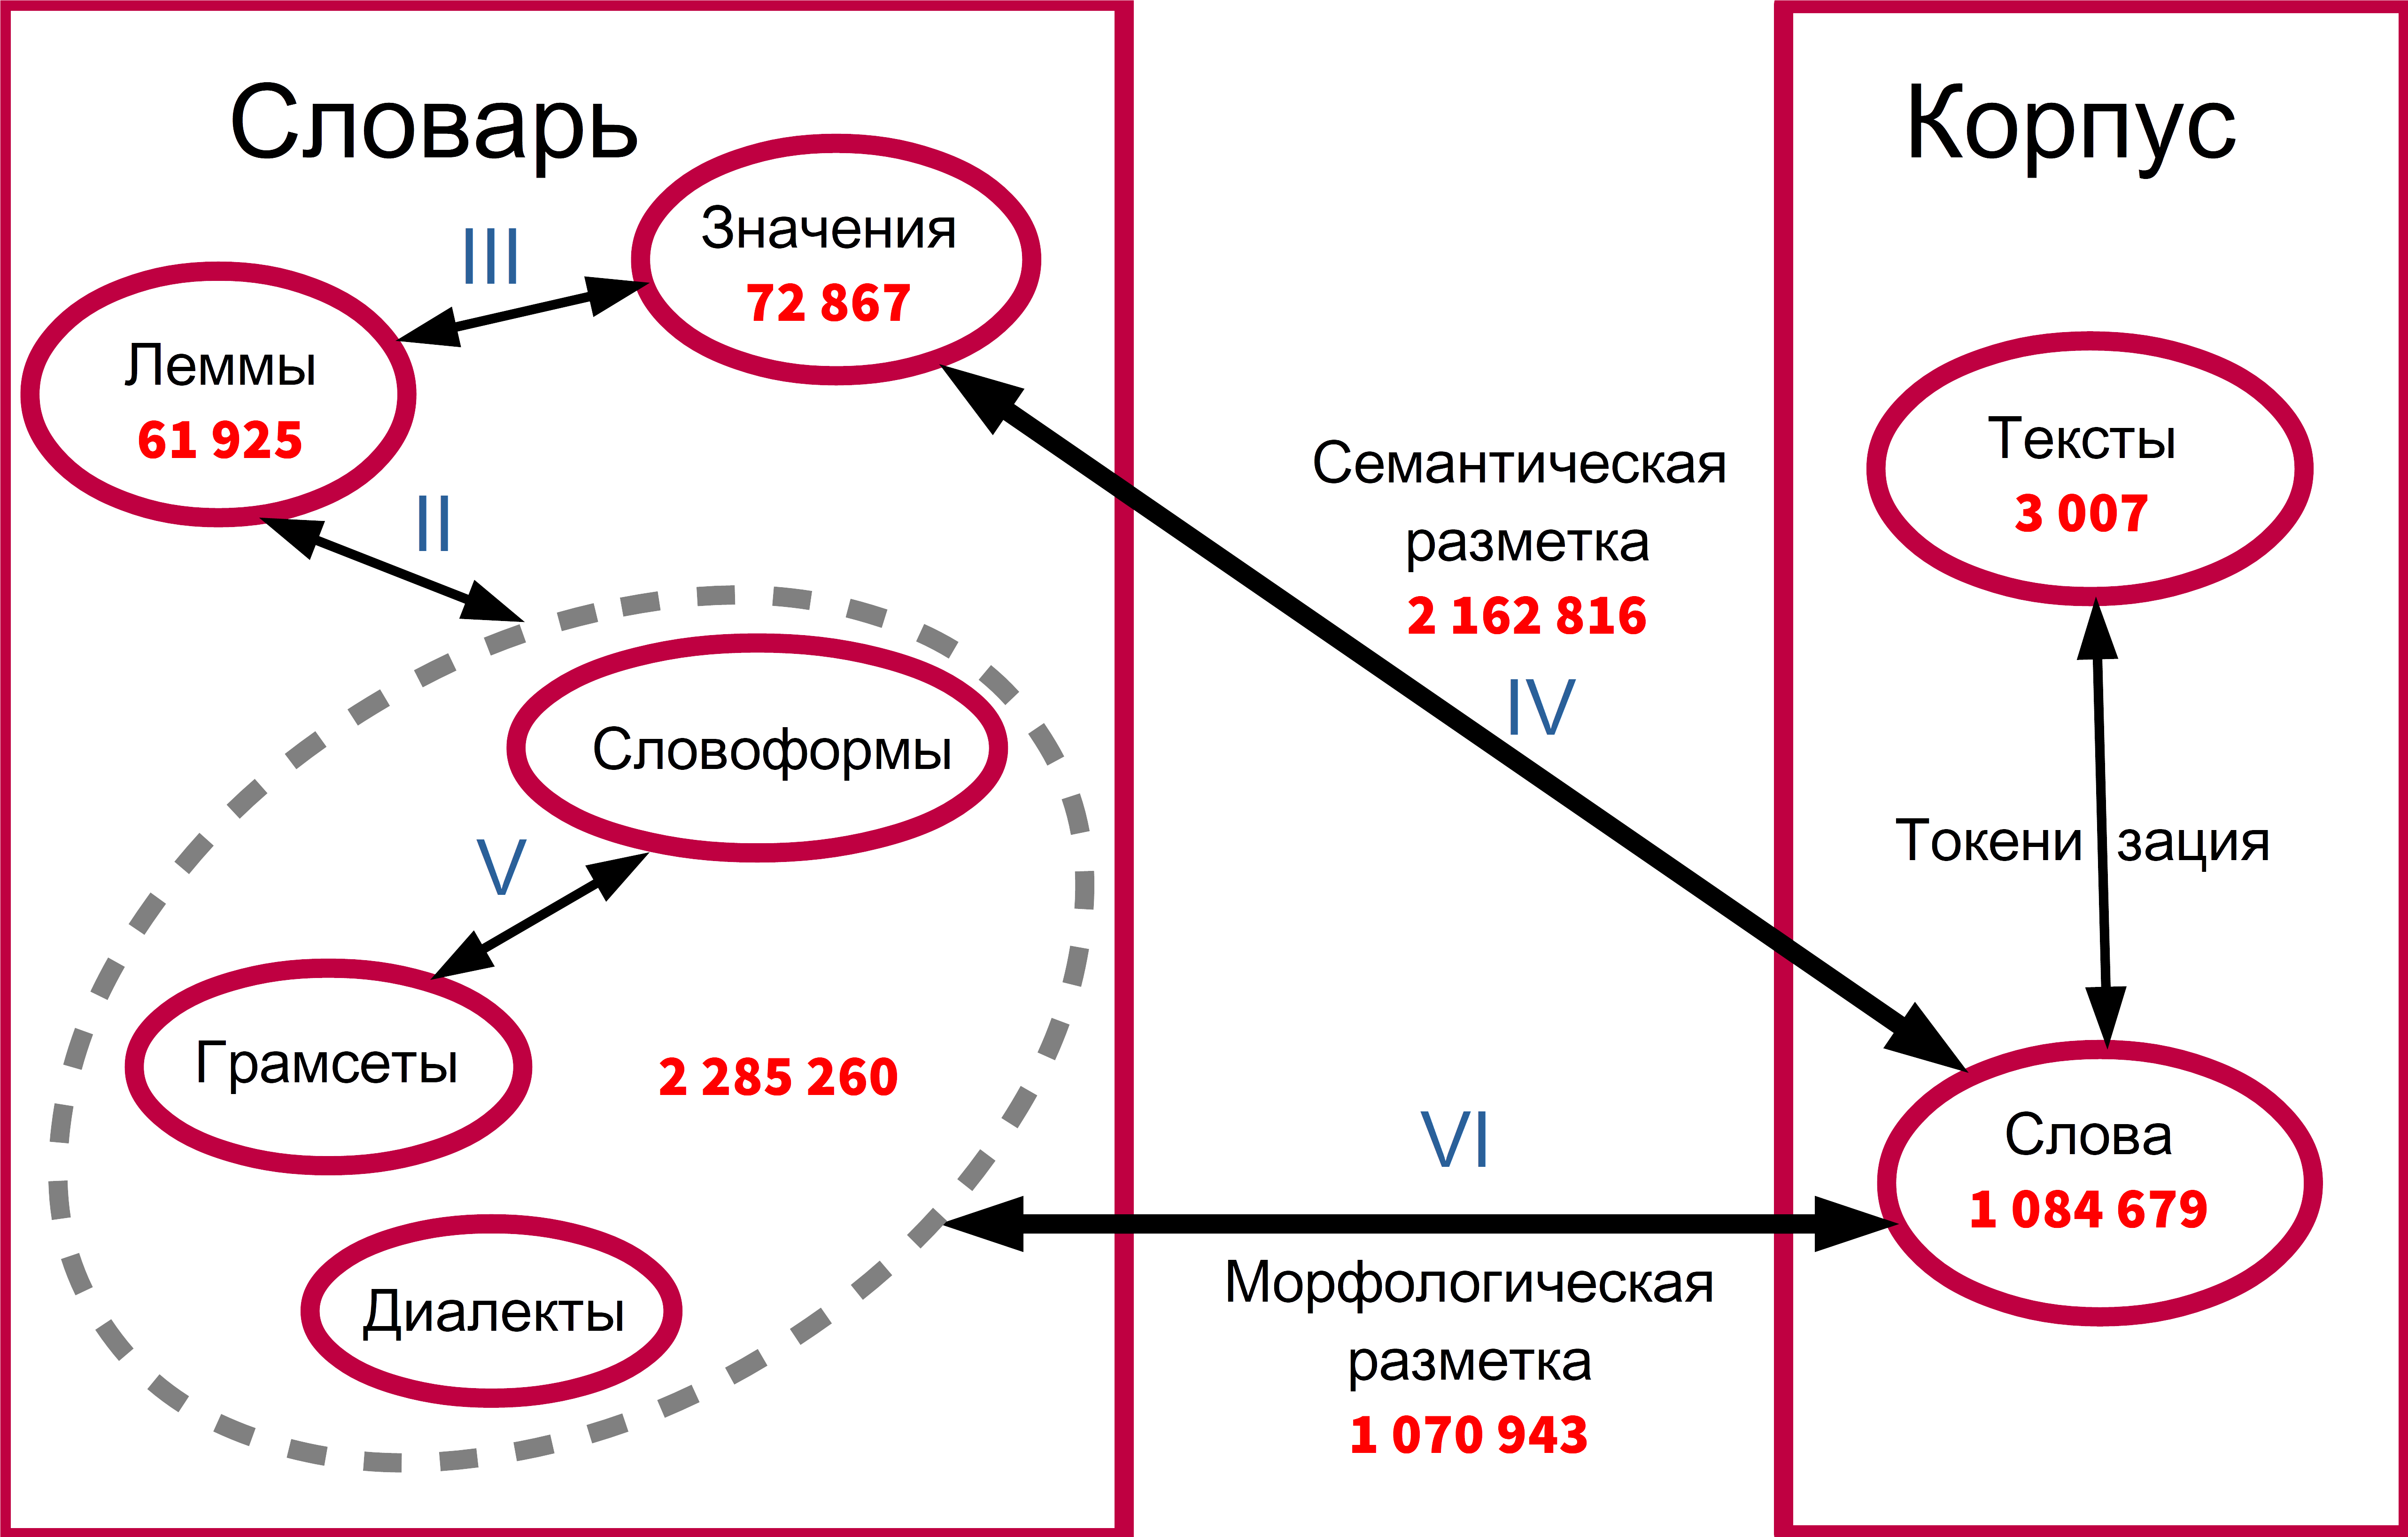
\includegraphics[width=1.0\textwidth,keepaspectratio=true]{corpus_manager_tagging.png}
\caption[Организация данных и разметка текста в корпуса ВепКар]{Организация 
данных и разметка текста в корпуса ВепКар, 
числовые данные приведены по всем языкам и диалектам. Данные на 10 февраля 2021 г.} \label{fig:corpus_manager_tagging}
\end{figure}

Проект ВепКар включает корпус текстов и связанный с ним словарь 
(рис.~\ref{fig:corpus_manager_tagging}). 
На февраль 2021 года в корпусе свыше 3000 текстов на 26 диалектах вепсского и карельского языков, свыше миллиона словоупотреблений. У некоторых текстов есть параллельный перевод на русский язык. Словарь корпуса содержит свыше 60 тысяч словарных статей со словоформами на 18 диалектах. Толкования слов в основном приводятся на русском и английском языках, хотя есть возможность давать толкования на вепсском, наречиях карельского и финском языках.

В текстах выделены границы предложений, в предложениях размечены слова (токены). 
Пример разметки:
\begin{lstlisting}[language=HTML]
<s id="17"><w id="141">Tulow</w> <w id="142">starikku</w> <w id="143">pertih</w>, <w id="144">tuattah</w> <w id="145">se</w>.</s>
\end{lstlisting}

Словарь включает леммы, связанные со значениями, и тройками словоформа--набор грамматических признаков (грамсет\footnote{ \textbf{gramset} -- \textbf{SET} of \textbf{GRAM}matical features})--диалект. 

Система ВепКар при разметке текста автоматически ищет в словаре 
леммы и словоформы, 
совпадающие в написании\footnote{При этом опускаются знаки смягчения (апострофы) 
и заменяются некоторых карельские буквы (в диалектных текстах встречаются буквы, 
которых нет в современном алфавите).
} 
с токенами. 
Это первый этап (\RNum{1}) разметки текста, не представленный на рис.~\ref{fig:corpus_manager_tagging}.  

\begin{enumerate}
\item \textbf{Семантическая разметка}. 
Для найденных в словаре словоформ выбираются связанные с ними леммы (\RNum{2} 
на рис.~\ref{fig:corpus_manager_tagging}), 
потом собираются все значения лемм (\RNum{3}) 
и устанавливаются семантические связи между словами из текста 
и значениями лемм (с пометкой <<не проверено>>) (\RNum{4}). 

%\begin{center}token (word) $\leftrightarrow$ word form $\leftrightarrow$ lemmas $\leftrightarrow$ meanings\end{center}

\begin{tikzpicture}
% TODO mbrace, examples:
% http://www.texample.net/tikz/examples/model-physics/
% http://www.texample.net/tikz/examples/assignment-structure/
% https://ipfs-sec.stackexchange.cloudflare-ipfs.com/tex/A/question/195131.html

%Nodes
\node (token)               {токены (слова)};
\node (wf) [right=of token] {словоформы};
\node (lemma) [right=of wf] {леммы};
\node (meaning) [right=of lemma] {значения};

%Lines
\draw[<->] (token.east) -- node[above] {\RNum{1}} (wf.west);
\draw[<->] (lemma.east) -- node[above] {\RNum{3}} (meaning.west);
\draw[<->] (wf.east) -- node[above] {\RNum{2}} (lemma.west);
\path[<->,red] (token.south) edge [bend right=13] node[above] {этап \RNum{4} не проверен} (meaning.south);
\end{tikzpicture}

%\begin{center}token (word) $\leftrightarrow$ word form $\leftrightarrow$ lemmas $\leftrightarrow$ meanings\end{center}

Задача эксперта-лингвиста~--- проверить эти связи и подтвердить их корректность, 
либо выбрать верную связь из нескольких возможных, 
либо вручную добавить новую словоформу, лемму или значение. 

Когда редактор (эксперт) кликает на токен в тексте, 
появляется выпадающий список всех значений найденных лемм. 
Редактор выбирает правильную лемму и значение (рис.~\ref{fig:text_tagging_by_editor}\footnote{
Полный текст доступен онлайн в корпусе ВепКар. 
См. страницу корпуса с этим текстом \url{http://dictorpus.krc.karelia.ru/en/corpus/text/494}.}). 

% samarialaine: http://dictorpus.krc.karelia.ru/en/corpus/text/494
% 
\begin{figure}
    \centering
    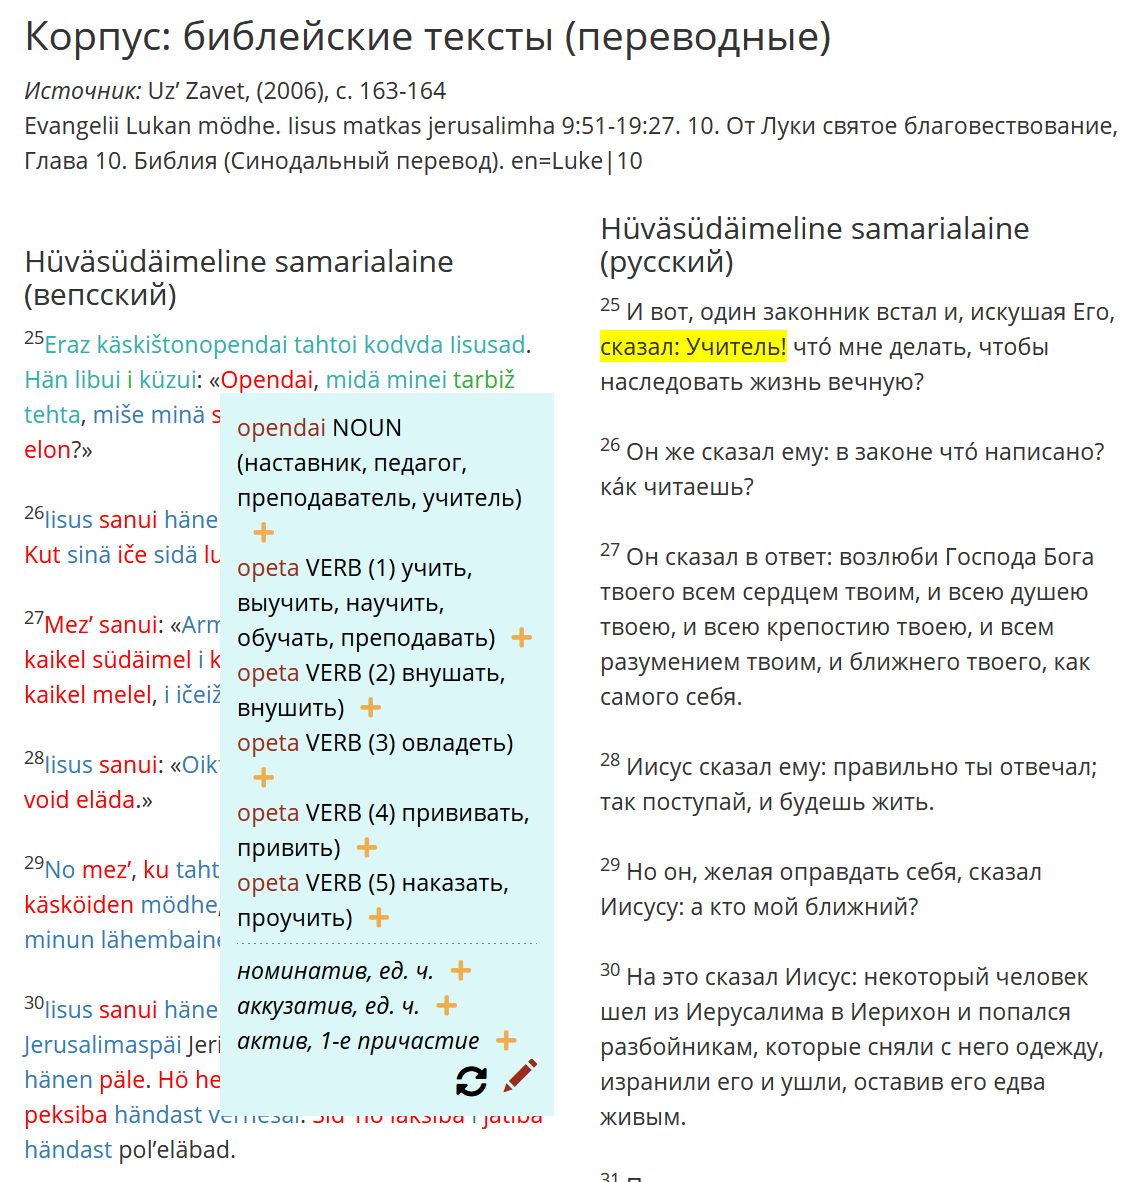
\includegraphics[width=1.0\textwidth,keepaspectratio=true]{text_tagging_by_editor.png}
\caption[Параллельный перевод текстов Библии]{Параллельный перевод текстов Библии: вепсский и русский языки. 
При клике в тексте по слову ``Opendai'' всплывает меню. 
Меню содержит значение для существительного <<учитель>> и пять значений для глагола. 
Когда редактор выбирает одно из значений, кликнув на знак $+$, 
то тем самым связывает токен и значение леммы ({\color{red}этап \RNum{4} проверен}).}
 \label{fig:text_tagging_by_editor}
\end{figure}

\item \textbf{Морфологическая разметка}. 
Для найденных словоформ выбираются связанные с ними грамсеты  (\RNum{5}) и устанавливаются морфологические связи (\RNum{6}) между словами из текста и парами ``словоформа — грамсет'' (Fig.~\ref{fig:text_tagging_by_editor}). 
Задача эксперта -- выбрать правильный грамсет.

\begin{tikzpicture}
%Nodes
\node (token)               {токены (слова)};
\node (wf) [right=of token] {словоформы};
\node (gramset) [right=of wf] {грамсеты};

%Lines
\draw[<->] (token.east) -- node[above] {\RNum{1}} (wf.west);
\draw[<->] (wf.east) -- node[above] {\RNum{5}} (gramset.west);
\path[<->,red] (token.south) edge [bend right=13] node[above] {\RNum{6}} (gramset.south);
\end{tikzpicture}

\end{enumerate}

Тексты корпуса автоматически размечены на 73\%, то есть для 790 тысяч слов в текстах система нашла соответствие в словаре: известны начальная форма (лемма), часть речи и другие морфологические признаки. Следующим этапом работы является работа экспертов по проверке разметки и снятию семантической (выбор значения) и морфологический (выбор грамматических признаков) омонимии.


Как отмечает Т. Архангельский для малоресурсных языков важно, чтобы при автоматическом морфологическом анализе сохранялись в разметке все возможные формы слова для последующей проверки и выбора правильной формы лингвистом~\cite[61]{Arkhangelskiy2020}. Архангельский Т. называет такой корпусный менеджер в корпусе «дружественным к неоднозначности», такой “ambiguity-friendly” платформой является при разметке корпус ВепКар.
%Следующим этапом работы является работа экспертов по проверке разметки и снятию семантической (выбор значения) и морфологический (выбор грамматических признаков) омонимии. 
Например, на рис.~\ref{fig:semantic_and_morph_omonymy} для карельского слова “missä” было найдено три значения местоимения “mi” (что; сколько, что; какой), одно значение наречия “missä” (где) и один набор грамматических признаков (инессив, ед. ч.; наречие - неизменяемое слово, без грамсетов). Для слова “muissa” было найдено одно значения глагола “muistua”, одно значение местоимения “muu” и три грамсета (одно для именной части речи и два для глагола). Эксперт кликая на иконку “плюс” выбирает правильное значение и правильный грамсет.

\begin{figure}
    \centering
    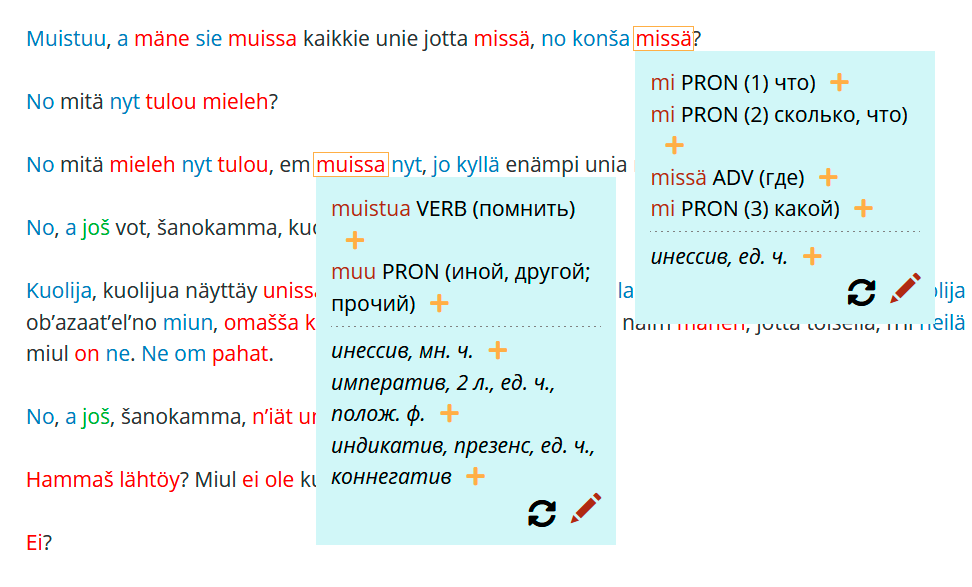
\includegraphics[width=1.0\textwidth,keepaspectratio=true]{vepkar_interface/semantic_and_morph_omonymy.png}
   \caption[Примеры семантической и морфологической омонимии в разметке текста корпуса ВепКар]{Примеры семантической и морфологической омонимии  в разметке текста корпуса ВепКар. 
Для карельского слова “missä” было найдено три значения местоимения “mi”, одно значение наречия “missä” и один грамсет. Для слова “muissa” было найдено одно значения глагола “muistua”, одно значение местоимения “muu” и три грамсета.} 
   \label{fig:semantic_and_morph_omonymy}
\end{figure}
 
\subsubsection{Особенности разметки корпуса ВепКар}\label{corpus_peculiarities}
В этом разделе опишем такую особенность разметки корпуса, из-за которой в описанных выше алгоритмах поиска не учитываются словоформы с пробелами и аналитические формы.
Aнaлитичecкaя фopмa – этo cocтaвнaя фopмa, oбpaзyeмaя coчeтaниeм вспомогательного и полнозначного слова.
Конечной целью настоящей работы является морфологическая разметка текста, предварительно разбитого на слова по пробельным и неалфавитным символам (например: скобки, знаки пунктуации, цифры). 
В имеющихся данных аналитические формы в тексте нам недоступны. 
Хотя в словаре мы храним полные парадигмы, в том числе и аналитические формы, в анализе текста подобные формы не участвуют, поскольку в тексте анализируется каждое отдельное слово, а не группа слов. 

Например, возьмем карельский глагол ‘pageta’ (уйти, убежать).
В словаре мы храним не только отрицательную форму 1 л. ед. ч. презенса индикатива: ‘en pagene’, но и коннегатив индикатива, презенс: ‘pagene’, который участвует в построении пяти из шести форм индикатива, презенс. 
Таким образом, в тексте будет размечено отдельно слово ‘en’ (вспомогательный глагол ‘ei’, индикатив, 1 л., ед. ч.) и отдельно ‘pagene’ (глагол ‘pageta’, коннегатив индикатива, презенс).
